% -------------------------------------------------------------------------------------------------
%      MDSG Latex Framework
%      ============================================================================================
%      File:                  introduction-[UTF8,ISO8859-1].tex
%      Author(s):             Michael Duerr
%      Version:               1
%      Creation Date:         30. Mai 2010
%      Creation Date:         30. Mai 2010
%
%      Notes:                 - Example chapter
% -------------------------------------------------------------------------------------------------
%
\chapter{Related Work}\label{sec:RelatedWork}
- Definition of field of research \\
- Scientific Scope \\
- Which comparable work in research exists? \\
- Separation from other works

\section{Credit Assignment Problem}
\marginpar{intro and comp. problems}
Realistic RL scenarios often involve multiple agents solving problems together, for example robots working in warehouses and factories. Such multiagent environments come with many difficulties. On one hand in a scenario where agents work independently it is very probable that they get in each other's way in order to score highest or finish a task, preventing the overall goal to be achieved.

\marginpar{coop problems}
In cooperative environments on the other hand, agents share the reward and therefore can not tell who contributed useful actions. Hence, all agents receive the same reward regardless of their contribution, which aggravates learning. The independence problem is discussed in chapter \ref{market} whereas the cooperation challenge is the focus point of this chapter.

\marginpar{coop and problem}
Sutton and Barto \cite{suba18} define a RL environment as cooperative, when agents execute their actions collectively each timestep but receive one overall reward in return. In this case individual learning is difficult or even impossible. Collective actions may contain bad choices that could be rewarded or, in case of a penalty, good actions that would be punished. Deciding which agent deserves more or less of the common reward is referred to as the credit assignment problem (CAP) \cite{mi61}.

\marginpar{CAP definition and kinds}
The CAP originated in a one-agent environment that only returned reward once the goal is reached or the terminating condition applied. A popular example of this is a chess game. In 1961, Minsky \cite{mi61} elaborated on this by explaining that a player wins or loses the game, but cannot retrace which decision got him there. Sutton later on decomposed the CAP into subproblems, namely the structural and temporal CAP \cite{su84}. He suggests, that the temporal CAP is assigning credit to each chess move by determining when the position improves or worsens, rewarding or penalizing that certain action. On the contrary, the structural CAP is assigning credit to the internal decision that leads to each particular action.

\marginpar{CAP multi}
% Sutton also refers to a chess game to explain the subproblems. 
Transferring the single-agent CAP into a multiagent environment Agogino and Tumer \cite{agtu04} imply that the problem shifts from being of temporal to structural type. They explain that while a single agent faces the temporal CAP due to many steps taken within an extended time period, in the multiagent case it becomes a structural CAP because of multiple actions in a single-time-step. Since the actions are executed all at once, the problem is now evaluating the decision that lies underneath.
% They explain that a single agent faces the temporal CAP when many steps are taken within an extended time period so learning from the returned reward at the end is problematic. Whereas in the multiagent setting it becomes a structural CAP because of multiple actions leading to a shared reward during a single-time-step.

\marginpar{cap solution dr}
Over the years many solutions and theories emerged in order to solve various CAP scenarios. An example for a simple approach is the difference reward (DR) \cite{agtu04},\cite{ngku18}. The idea is to calculate the reward with the joint multiagent actions as always. In every step however, each agent decomposes that reward by calculating the difference between a new reward and the old one. The new reward is generated with the same actions, only modifying the action of the current agent, setting it to a default or waiting value. With this method each agent has the opportunity to learn how they contributed to the resulting state and reward, enabling individual learning. High DR values indicate lucrative actions of the analyzing agent. The opposite case applies for low valued DRs.

\section{Markets}\label{market}
\marginpar{intro mixed motive}
As described earlier, agents that share an environment and act independently can often hinder each other from reaching the common or individual goal. Sutton and Barto defined a game to be competitive, when agents receive varying reward signals \cite{suba18}. In most cases agents follow a mixed-motive, meaning that their individual rewards could sometimes align and sometimes be in conflict. An environment is purely competitive, when the increase in reward of one agent leads to reward decrease of the others.

\marginpar{SMG details}
Schmid et al. introduced in ``Stochastic Market Games'' \cite{scbe21} concepts adding incentives when agents act cooperatively in mixed-motive settings to improve the overall rewards for all participants. The idea of a Stochastic Market Game (SMG) is to enable dominant cooperative strategies through a global and impartial trading market. A stochastic game becomes a SMG if two conditions are met. First, the environment actions of agents are extended with market actions. Second, the reward function adjusts the calculated rewards based on agreements met in the market executions. Furthermore Schmid et al. defined two types of markets: unconditional and conditional markets.

\marginpar{sm}
They compare the concept of unconditional markets to companies and shareholders, since shareholders do not need to fulfill any conditions to receive the dividends. In unconditional SMGs both companies and shareholders are agents that buy and sell shares as market actions. Figure \ref{fig:sm} shows such a shareholder market (SM). Each timestep every agent has the possibility to put their share on the market or to announce a buying offer directed to another agent.

\marginpar{sm transaction}
If the buying offer coincide with a share that is up for sale in the same timestep, a market transaction is registered. From there on out the shareholder participates in the reward of the transaction agent by a fixed dividend $d$. Schmid et al. mention that an optional price $p$ can be defined as a price a seller receives from the buyer upon each share purchase. They claim however, that agents with high rewards are very likely to gift their shares in order to align the goals of the other agents with their own. Shareholders profit from the success of the selling party through the dividends.

\marginpar{am}
On the contrary, the authors define conditional markets similar to purchase contracts, where buyers pay a fixed price $p$ to sellers when they in turn meet the buyers demand. A proposed conditional SMG is the so called action market (AM). In this case actions are extended with a buying offer, containing one expected action from one specific agent, see figure \ref{fig:am}.

% Illustations of conditional and unconditional markets, as defined in ``Stochastic Market Games''\cite{scbe21}}
% \label{fig:multipic}

\begin{figure}[hpbt]
    \centering
    %%----start of first subfigure----
    \subfloat[Shareholder market (taken from ``Stochastic Market Games''\cite{scbe21})]{
        \label{fig:sm} %% label for first subfigure
        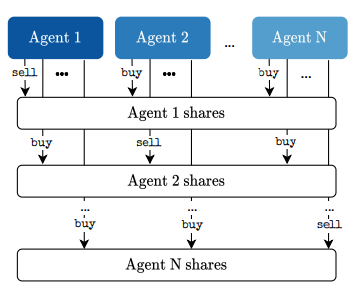
\includegraphics[width=0.48\linewidth]{pictures/SMG_sm.png}}
    \hspace{0.01\textwidth}
    %%----start of second subfigure----
    \subfloat[Action market]{
        \label{fig:am} %% label for second subfigure
        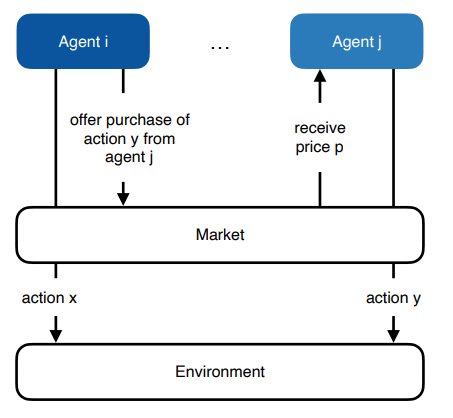
\includegraphics[width=0.41\linewidth]{pictures/SMG_am.png}}
    \caption[Illustrated Markets]{Illustrated Markets as defined in ``Stochastic Market Games''\cite{scbe21}}
    \label{fig:multipic} %% label for entire figure
\end{figure}

\marginpar{am transaction}
A purchase is established if the specified agent happens to execute the environment action the buyer expected. It is important to emphasize that the matching happens during one timestep, leaving it to chance, whether purchases take place. Hence, agents do not know in advance if and what action another agent could be buying from them. Despite this uncertainty, the researchers showed, that both market implementations yielded promising results. An increase of the overall rewards of participating agents in mixed-motive games was seen.